%************************************************
\chapter{Kernfaktoren einer sozialen Netzwerkanalyse}\label{ch:kernfaktoren} % $\mathbb{ZNR}$
%************************************************
In komplexen Netzwerken können einige Knoten als wichtiger angesehen werden als andere. In einem sozialen Netzwerken zeichnen sich wichtige Knoten durch vergleichsweise mehr Verbindungen als andere Knoten aus. Auf das Beispiel \textit{Instagram} bezogen, können solche Knoten Informationen gut verbreiten, sogenannte Influencer. Daher werden diese Knotenpunkte als zentral oder sozial wichtig interpretiert. Die Interpretation der Zentralität ist jedoch nicht eindeutig \cite{GOLBECK201325}. Zum Beispiel im Linienverkehr,
gilt eine Linie als zentral, wenn sie von großen Menschenmengen genutzt und stärker frequentiert wird,
als andere Linien. Die Definition der Zentralität ist also nicht allgemein und hängt von der Anwendung ab. Da es keine allgemeine Definition von Zentralität gibt, wurden mehrere Maße entwickelt, die jeweils spezifische Konzepte berücksichtigen.
Die Zentralität ist deshalb eine Schlüsseleigenschaft komplexer Netzwerke. Sie kann unter anderem das Verhalten dynamischer Prozesse wie beispielsweise eine epidemische Ausbreitung erklären, modellieren und abschätzen, jedoch nicht beschreiben, da es oftmals schwierig ist exakte Aussagen zu tätigen, wenn unbekannte Faktoren in den Datensätzen enthalten sind. \cite{SpringerElbert}. Zudem kann die Zentralität Informationen über die Organisation komplexer Systeme und unsere Gesellschaft liefern. Es gibt viele Metriken zur Quantifizierung der Knotenzentralität in Netzwerken \cite{francisco}.

\section{Zentralitäten}
\label{ch:Zentralitaeten}
Die \textit{Grad-Zentralität} ist die am einfachsten zu berechnende Zentralität. Sie ist definiert durch die Anzahl der \textit{direkten} Verbindungen eines Knoten. Mit der Adjazenzmatrix wird der Grad der Zentralität berechnet, indem die Summe der Elemente der betroffenen Zeile $i$ berechnet wird.
Mathematisch formuliert, wird folgende Formel verwendet: 
\begin{equation}
     k_i &= \sum_{j=1}^{N} A_i_j 
     \label{degree}
\end{equation}

Wobei $A$ die Adjazenzmatrix beschreibt, $N$ die Anzahl an Knoten darstellt und $i$, $j$ die Knoten. \\
Da es sich bei der \textit{Grad-Zentralität} um die einfachste Zentralität handelt, wird meist davon ausgegangen, dass Knoten mit vielen Verbindungen, daher mit einer hohen Zentralität, sich visuell betrachtet im Zentrum eines Netzwerkers befinden. Dies hat jedoch einige Nachteile, denn Knoten mit der höchsten \textit{Grad-Zentralität} können sich auch visuell am Rand des Netzes befinden, was dazu führt, dass die \textit{Grad-Zentralität} nicht als lokales Maß betrachtet wird. Zudem sollte hervorgehoben werden, dass bei der \textit{Grad-Zentralität} nur ein- beziehungsweise ausgehende Kanten gezählt werden. Dies sagt zwar aus, dass ein solcher Knoten, auf das soziale Netzwerk bezogen, eine beliebte oder sehr bekannte Person ist, doch es ist dadurch keine Aussage über die Macht oder den Einfluss der Person möglich. Als extremes Beispiel, warum die \textit{Grad-Zentralität} nicht immer optimal zur Netzwerkanalyse ist, diene ein Netzwerk mit einer großen, dichten Gruppen von Knoten. Als dichte Gruppe ist hierbei eine Ansammlung von Knoten zu verstehen, welche sich alle nah beieinander befinden. Diese machen den größten Teil des Graphen aus, welcher auch als Kern des Netzes bezeichnet wird. Jedoch kann (visuell betrachtet) weit außerhalb des Kerns, entlang einer Kette von Knoten mit niedrigem Grad, ein Knoten liegen, welcher mit einer großen Anzahl von Knoten verbunden ist. Ein solcher Knoten hätte einen hohen Grad an Zentralität, obwohl er weit vom Kern des Netzes und den meisten Knoten entfernt ist \cite{SpringerElbert}. 
Um solche Faktoren mit berücksichtigen zu können, wird ein weiterer Faktor in die Berechnung integriert, nämlich die Weglänge. \\

Diese spielt eine wichtige Rolle bei der \textit{Nähe-Zentralität}, 
denn die Knotenzentralität kann auch anhand der kürzesten Wege definiert werden. Der Abstand zwischen zwei Knoten $i$ und $j$ ist gegeben durch die Anzahl der Kanten, welche sie möglichst direkt verbindet. Ein zentraler und daher wichtiger Knoten liegt, bezogen auf den Abstand, nahe an allen anderen Knoten des Netzes. Dieser Gedanke ist im Maß der sogenannten \textit{Nähe-Zentralität} oder \textit{Closeness-Centrality} enthalten. Diese wird durch den durchschnittlichen Abstand eines jeden Knotens zu allen anderen Knoten definiert. Mathematisch wird die Formel wie folgt beschrieben: 

\begin{equation}
     C_i &= \frac{N}{\sum_{j=1, j \not{=}i}^{N} d_i_j }
\end{equation}

Dabei ist mit $d_i_j$ der kürzeste Weg zwischen $i$ und $j$ gemeint und mit $N$ erneut die Anzahl an Knoten im Netzwerk \cite{SpringerElbert}. Die \textit{Nähe-Zentralität} ist vor allem dann sehr geeignet, wenn Prozesse über kurze Wege charakterisiert werden sollen. Beispielsweise kann der hierarchischen Aufbau eines Unternehmens in einem sternförmigen Graphen dargestellt werden. In der Mitte des Graphen befindet sich der Vorstand, der in engem Kontakt mit den jeweiligen Abteilungsleitern steht. Die Abteilungsleiter sind, neben dem Vorstand, wiederum in sehr nahem Kontakt mit ihren jeweiligen Mitarbeitern ihrer Abteilung. Wenn nun ausschließlich anhand der \textit{Grad-Zentralität} argumentiert wird, sind die Abteilungsleiter die wichtigsten Knoten im Graphen. Jedoch haben diese nicht die niedrigste \textit{Nähe-Zentralität}, denn der Vorstand hat, da sich dieser Knoten visuell in der Mitte des Graphen befindet, zu allen anderen Knoten entweder einen oder zwei Kanten Abstand. Die einzelnen Abteilungsleiter haben aber, im worst-case Fall, zu anderen Angestellten aus anderen Abteilungen zwei bis drei Kanten Abstand. Dementsprechend ist es nicht ausreichend nur eine Zentralität bei der Analyse von \textit{sozialen Netzwerken} zu betrachten. Bei der \textit{Nähe-Zentralität} weisen die meisten komplexen Netze eine geringe durchschnittliche Länge des kürzesten Weges auf. Dies ist damit zu begründen, dass die durchschnittliche Entfernung mit dem Logarithmus über die Anzahl der Knoten zunimmt. 
Daher liegt das Verhältnis zwischen dem größten und dem kleinsten Abstand
in der Größenordnung $log(N)$, da der minimale Abstand gleich eins ist. In den meisten real existierenden
Netzwerken beträgt dieses Verhältnis etwa 6 oder weniger. Es kann also mehrere Knoten mit der gleichen
Zentralität geben, obwohl sie bei der Informationsverbreitung unterschiedliche Rollen spielen können. Daher ist die \textit{Nähe-Zentralität} besser geeignet für räumliche Netze, bei denen die Abstände zwischen den Knoten größer sind als in zufälligen Netzen mit der gleichen Anzahl von
Knoten und Verbindungen \cite{SpringerElbert}.\\

\newpage
Die \textit{Betweenness-} oder \textit{Zwischen-Zentralität} hingegen misst, wie wichtig ein Knoten für die kürzesten Pfade durch das Netz ist. Um diese Zentralität für einen Knoten $N$ zu berechnen, wird in dieser Methode eine Gruppe von Knoten ausgewählt und alle kürzesten Wege zwischen diesen Knoten gesucht. Dann wird der Anteil dieser kürzesten Wege berechnet, die den Knoten $N$ einschließen. Wenn es beispielsweise 7 kürzeste Wege zwischen einem Knotenpaar gibt und 5 davon durch den Knoten N führen, dann wäre der Anteil $5/7=0.714$. Dieser Vorgang wird für jedes Knotenpaar im Netz wiederholt. Anschließend werden die berechneten Brüche addiert, wodurch die \textit{Zwischen-Zentralität} des Knotens $N$ generiert wird. Mathematisch formuliert sieht die Formel dann wie folgt aus: 
\begin{equation}
     B_i &= \sum_{(a-b)}\frac{\eta(a,i,b)}{\eta(a,b)}
\end{equation}
Hierbei bezeichnet $\eta(a,i,b)$ die Anzahl der kürzesten Wege zwischen den Knoten $a$ und $b$ die durch den Knoten $i$ führen. Zudem stellt $\eta(a,b)$ die Gesamtzahl der kürzesten Wege zwischen $a$ und $b$ dar. 
Diese Zentralität, basierend auf dem \textit{random walk-Algorithmus} und ist gegeben durch die erwartete Anzahl der Besuche von jedem Knoten $i$ während einer zufälligen Schrittfolge durch den Graphen:
\begin{equation}
     B_i &= \sum_{a=b}^{N}\sum_{b=1}^{N}w(a,i,b)
\end{equation}
dabei ist $w(a,i,b)$, wie oben bereits beschrieben für $\eta(a,i,b)$, die Anzahl der kürzesten Wege zwischen den Knoten $a$ und $b$, die durch den Knoten $i$ führen. Die Lösung wird daher nur angenähert.
Die \textit{Zwischen-Zentralität} ist eines der am häufigsten verwendeten Zentralitätsmaße. Sie gibt an, wie wichtig ein Knoten für den Informationsfluss von einem Knoten des Netzes zu einem anderen ist. In gerichteten Netzwerken kann die \textit{Zwischen-Zentralität} mehrere Bedeutungen haben \cite{SpringerElbert}. Einem Nutzer $Anton$ mit hoher \textit{Zwischen-Zentralität} folgen möglicherweise viele andere Nutzern, welche jedoch nicht denselben Personen folgen wie der Nutzer $Anton$ selbst. Dies würde darauf hindeuten, dass der Nutzer $Anton$ viele Anhänger oder Follower hat. Es kann aber auch sein, dass der Nutzer $Anton$ weniger Follower hat, diese aber dafür mit vielen Knoten verbindet, die ansonsten weit entfernt sind. Daher ist es enorm wichtig die Richtung der Kanten eines Knotens zu kennen, um die Bedeutung der Zentralität zu verstehen. \\

Die \textit{Eigenvektor-}oder \textit{Eigenwert-Zentralität} misst die Bedeutung eines Knotens, wobei die Bedeutung seiner Nachbarn berücksichtigt wird. Deshalb wird sie manchmal verwendet, um den Einfluss eines Knotens im Netzwerk zu messen. Sie wird durch eine Matrixberechnung ermittelt, um den so genannten \textit{Haupteigenvektor} anhand der Adjazenzmatrix zu bestimmen. Mathematisch betrachtet ist die \textit{Eigenvektor-Zentralität} die komplizierteste, der in dieser Arbeit betrachteten Zentralitäten.\\
Wird nun die Tatsache betrachtet, dass ein Akteur zentraler ist, wenn er in Beziehung zu weiteren Akteuren steht, die selbst zentral sind, so kann argumentiert werden, dass die Zentralität eines Knotens nicht nur von der der Anzahl seiner Nachbarknoten abhängt, sondern auch von deren Zentralitätswert. Beispielsweise definiert Bonacich (1972) die Zentralität $c(v_i)$ eines Knotens $v_i$ als positives Vielfaches der Summe der benachbarten Zentralitäten. Als Formel mathematisch dargestellt sieht dies folgendermaßen aus:
\begin{equation}
     \lambda c(v_i) = \frac{1}{\lambda} \sum_{j=1}^{N}a_{ij}c(v_j) \forall i
\end{equation} oder umformuliert:  
\begin{equation}
     c(v_i) = \sum_{j=1}^{N}a_{ij}c(v_j) \forall i
\end{equation}
Hierbei repräsentiert $a_{i,j}$ die Werte der Adjazenzmatrix $A$ und $\lambda$ einen konstanten Faktor. \\
In Matrixschreibweise mit $c = (c(v_1), ...., c(v_n))$ bedeutet dies auch:
\begin{equation}
     Ac = \lambda c
\end{equation}
Diese Art von Gleichung wird durch die Eigenwerte und Eigenvektoren von $A$ gelöst.
Aus der gesamten Menge an verschiedenen Eigenvektoren, soll es nur eine geeignete Lösung geben. 
Dieser Eigenvektor kann dann direkt als Zentralitätsmaß dienen. Da $A$ die Adjazenzmatrix eines ungerichteten (zusammenhängenden) Graphen ist, ist $A$ nicht negativ und aufgrund des Satzes von Perron-Frobenius, existiert ein Eigenvektor des maximalen Eigenwerts mit ausschließlich nicht negativen, also positiven, Einträgen \cite{brittaRuhnau}.

\section{Cliquen und Brücken}
\label{ch:CliquenBrücken}
Eine Clique ist laut Definition ein Teilgraph, aus mindestens drei Knoten bestehend, die zudem alle benachbart zueinander sind. Streng bezeichnet handelt es sich bei einer Clique um eine zusammenhängende Untergruppe. Eine Clique kann ebenso als Ansammlung von Akteuren gesehen werden, die sich gegenseitig wählen, jedoch wählt kein anderer Akteur dieser Gruppe weitere Akteure aus weiteren Gruppen und wird auch nicht von anderen Akteuren gewählt. Es ist zu beachten, dass sich Cliquen in einem Graphen auch überlappen können, also derselbe Satz von Knoten zu mehr als nur einer Clique gehören kann. Zu beachten ist, dass eine vollständige Clique nicht in einer anderen Clique enthalten sein kann, denn sonst wäre die kleinere Clique nicht mehr maximal. Die Cliquendefinition ist vor allem nützlich, für die Untersuchung der Eigenschaften einer Untergruppe beziehungsweise eines Subgraphen \cite{wasserman1994social}. Was genau damit gemeint ist, ist in folgendem Plot zu sehen: 
\FloatBarrier
\begin{figure}[htb!]
    \centering
    %\hspace*{-1cm}
    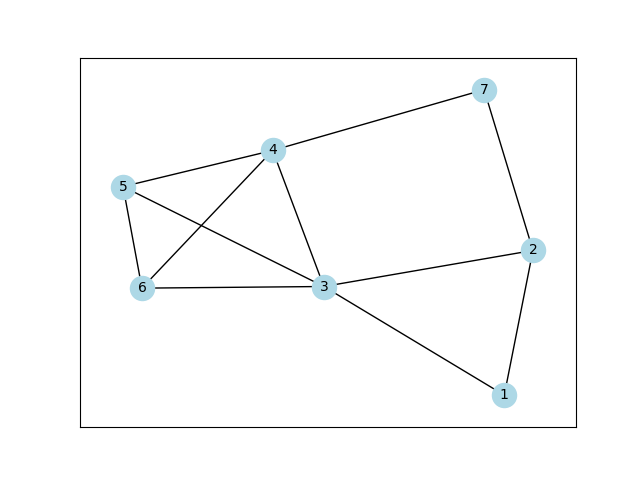
\includegraphics[width=0.55\textwidth]{Graphics/Clique.png}
    \caption{Graph mit den Cliquen (1, 2, 3) und (3, 4, 5, 6)}
    \label{fig:Clique}
\end{figure}

\newpage
Wichtig ist hierbei, dass es sich bei (2, 3, 4, 7) um keine Clique handelt, da keine Verbindung zwischen den Knoten \textbf{4 und 2} und ebenso keine Verbindung zwischen den Knoten \textbf{3 und 7} besteht.
Neben den Cliquen sind auch Brücken eine wichtige Diskussions- und Analysierungsgrundlage für Graphen beziehungsweise in unserem Fall für \textit{soziale Netzwerke}. Wenn von Brücken (bzw. englisch Bridge) die Rede ist, sind Verbindungen zwischen zwei Knoten gemeint. Jedoch handelt es sich um die einzige Verbindung zwischen diesen Knoten und deren Kontakten \cite{bridge}. Ein Beispiel für Brücken im Graphen liefert folgender Plot:

\FloatBarrier
\begin{figure}[htb!]
    \centering
    %\hspace*{-1cm}
    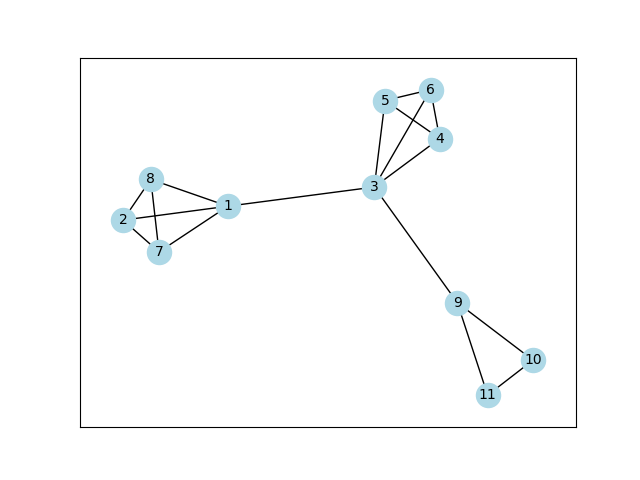
\includegraphics[width=0.55\textwidth]{Graphics/Bridge.png}
    \caption{Graph mit den Brücken (1, 3) und (3, 9)}
    \label{fig:Bridge}
\end{figure}
Hierbei ist gut zu erkennen, dass die drei Subgraphen durch \textit{Brücken} miteinander verbunden sind. Neben den Brücken sind in Abbildung \ref{fig:Bridge} die Cliquen (1,2,7,8), (3,4,6,5) und (9,10,11) enthalten. Zu beachten ist, dass es sich bei beispielsweise (1,7,8) oder (4,5,6) um keine Cliquen handelt. Wenn nun diese Brücken und Cliquen im Zusammenhang mit den Zentralitäten betrachtet werden und die oben aufgeführten Formeln der Zentralitäten auf den Graphen \ref{fig:Bridge} angewendet werden, erhält man die unten stehende Tabelle \ref{table:TableCliqueBridg}. Eine Berechnung für Abbildung \ref{fig:Clique} ist nicht nötig, da in Abbildung \ref{fig:Bridge} ebenfalls Cliquen und zusätzlich Brücken enthalten sind:
\begin{table}[h!]
\centering
\footnotesize
\caption{Werte Abbildung \ref{fig:Bridge}}
\label{table:TableCliqueBridg}
\begin{tabular}{lccccc}\toprule
\textbf{Node} & \textbf{Grad-Zentr.} &\textbf{Nähe-Zentr.} &\textbf{Betweeness-Zentr.} & \textbf{Eigen.-Zentr.} \\
 &\\\midrule
  3 & 0.5 & 0.666667 & 0.733333 & 0.470733  \\
  1 & 0.4 & 0.555556 & 0.466667 & 0.387253  \\
  4 & 0.3 & 0.454545 & 0        & 0.340195  \\
  6 & 0.3 & 0.454545 & 0        & 0.340195  \\
  5 & 0.3 & 0.454545 & 0        & 0.340195  \\
  2 & 0.3 & 0.4      & 0        & 0.279871  \\
  7 & 0.3 & 0.4      & 0        & 0.279871  \\
  8 & 0.3 & 0.4      & 0        & 0.279871  \\
  9 & 0.3 & 0.5      & 0.355556 & 0.184986  \\
 10 & 0.2 & 0.357143 & 0        & 0.0776041 \\
 11 & 0.2 & 0.357143 & 0        & 0.0776041 \\
       
  \\\bottomrule
 \end{tabular}
 \end{table}

Direkt fällt auf, dass die Werte spaltenweise sehr ähnlich zueinander sind. Bei der \textit{Gradzentralität} sind die Knoten \textbf{3} und \textbf{1} mit einem Wert von \textbf{0.5} und \textbf{0.4} am höchsten. Interessant, denn dabei handelt es sich um die Knoten, die unsere \textit{Brücke} bilden. Bei den Knoten \textbf{3} und \textbf{1} fällt des weiteren auf, dass diese Knoten bei der \textit{Nähe-}, \textit{Zwischen-} und \textit{Eigenvektor-Zentralität} ebenfalls am höchsten sind. Das heißt, die Vermutung liegt nahe, dass die Knoten eines Graphen, die Cliquen bilden, relativ ähnliche \textit{Zentralitätswerte} aufweisen beziehungsweise die Varianzen geringer sind. Aber vor allem erwähnenswert ist, dass in der Tabelle \ref{table:TableCliqueBridg} lediglich bei den Knoten, welche die \textit{Brücke} bilden, Werte ungleich \textit{Null} in der Spalte \textit{Betweeness-Zentr.} auffindbar sind. Dies sollte für den weiteren Teil der Arbeit in Erinnerung bleiben. 


\section{Soziale Netzwerk-Eigenschaften}
\label{ch:eigenschaftenTabelle}
Die wichtigsten Eigenschaften eines sozialen Netzwerks sind die folgenden: 
\begin{table}[h!]
\footnotesize
\caption{Eigenschaften eines sozialen Netzwerks}
\label{TableEigenschaften}
%\centering
\begin{tabular}{lcc}\toprule 
\textbf{Eigenschaft} &\textbf{Beschreibung} \\
 &\\\midrule
 \\
  \textbf{Cluster} & Ein soziales Netzwerk sollte aus mehreren Cluster oder Subgraphen \\ &bestehen. Diese können in ihrer Größe und Anzahl stark variieren   \\
  \\
  \textbf{Brücke} & Die einzelnen Cluster sind über Brücken miteinander verbunden \\
  \\
  \textbf{Clique} & In den Cluster sollten Cliquen vorzufinden sein, d.h mindestens \\
  & drei Knoten existieren die untereinander alle miteinander verbunden sind \\
  \\
  \textbf{Grad-Zentralität} &  Die einzelnen Knoten der Cluster sollten unterschiedliche Grad-\\
  & Zentralitäten haben. Hohe Zentralitäten bedeuten, dass es sich \\
  & um wichtige Knoten handelt, niedrige Werte, dass es weniger \\ 
  & wichtige Knoten sind. Wichtig ist jedoch, dass es nicht aus-\\
  & schließlich wichtige oder ausschließlich unwichtige Knoten gibt.  \\
  \\
  \textbf{Nähe-Zentralität} & Auch hier sollen die Knoten im Cluster unterschiedliche Wert \\
  & aufweisen. Hohe Werte bedeuten, die Knoten sind nah bei- \\
  & einander, haben kurze Wege zueinander. Niedrige Werte \\
  & bedeuten, dass die Knoten weite Entfernungen zueinander haben.\\
  \\
  \textbf{Zwichen-Zentralität} & Hier wird die Wichtigkeit der Nachbar-Knoten in Relation \\
  & bewertet. Hohe Werte bedeuten, dass diese Knoten oft \\
  &für den kürzesten Weg verwendet werden. Niedrige Werte, \\
  & dass diese Knoten nicht für die kürzesten Wege relevant sind.\\
  
  \\\bottomrule
 \end{tabular}
 \end{table}
Natürlich gibt es deutlich mehr Faktoren als die in Tabelle \ref{TableEigenschaften} dargestellten. Jedoch sind diese die primären Eigenschaften, welche in dieser Arbeit berücksichtigt werden.
Nun sind die wichtigsten Eigenschaften der, in dieser Arbeit betrachteten und verwendeten, Metriken wie Clique, Größe oder Brücken bekannt und eingeführt. Manche Zentralitäten wurden oberflächlicher erklärt als andere, weil sie weniger relevant für die Untersuchung der sozialen Netzwerke sind. In Zukunft wird in dieser Arbeit bei \textit{typischen Eigenschaften} von Netzwerken stets auf Tabelle \ref{ch:eigenschaftenTabelle} verwiesen.

\newpage
\section{Ein typisches soziales Netzwerk}
Nachdem nun alle Zentralitäten, deren Berechnungen und weitere wichtige Eigenschaften von sozialen Netzwerken bekannt sind, ist es an der Zeit ein Musterbeispiel für ein soziales Netzwerk zu betrachten. Das bekannteste Netzwerk ist natürlich Facebook. Bei dieser sozialen Plattform ist die geeignetste Darstellung ein \textit{ungerichteter} Graph. Bei Instagram hingegen, ein \textit{gerichtet} Graph. Denn hier gibt es neben Leuten, denen wir folgen, die eigenen Follower \cite{fbInsta}. Die Knoten sind sogenannte \textit{Nutzer} und die \textit{Kanten} sind Verbindungen zwischen ihnen. Zu beachten ist, dass sowohl \textit{Knoten} als auch \textit{Kanten} Attribute zugewiesen werden können. Knotenattribute in Facebook können zum Beispiel \textit{Geschlecht}, \textit{Ort}, \textit{Alter} usw. sein, und Kantenattribute können \textit{Datum der letzten Unterhaltung zwischen zwei Knoten}, \textit{Anzahl der Likes}, \textit{Datum der Verbindung} usw. sein \cite{GOT}.
Im folgenden wird ein, auf den ersten Blick und nach den Eigenschaften von \\ 
Tabelle \ref{ch:eigenschaftenTabelle} typisch erscheinendes, soziales Netzwerk betrachtet. Es muss jedoch stets klar sein, dass es sich hierbei um den Datensatz eines fiktiven Fantasy Drama handelt \cite{GOT} und es daher zu Unstimmigkeiten bei den Ergebnissen und der Analyse kommen kann.

\FloatBarrier
\begin{figure}[h!]
    \centering
    %\hspace*{-1cm}
    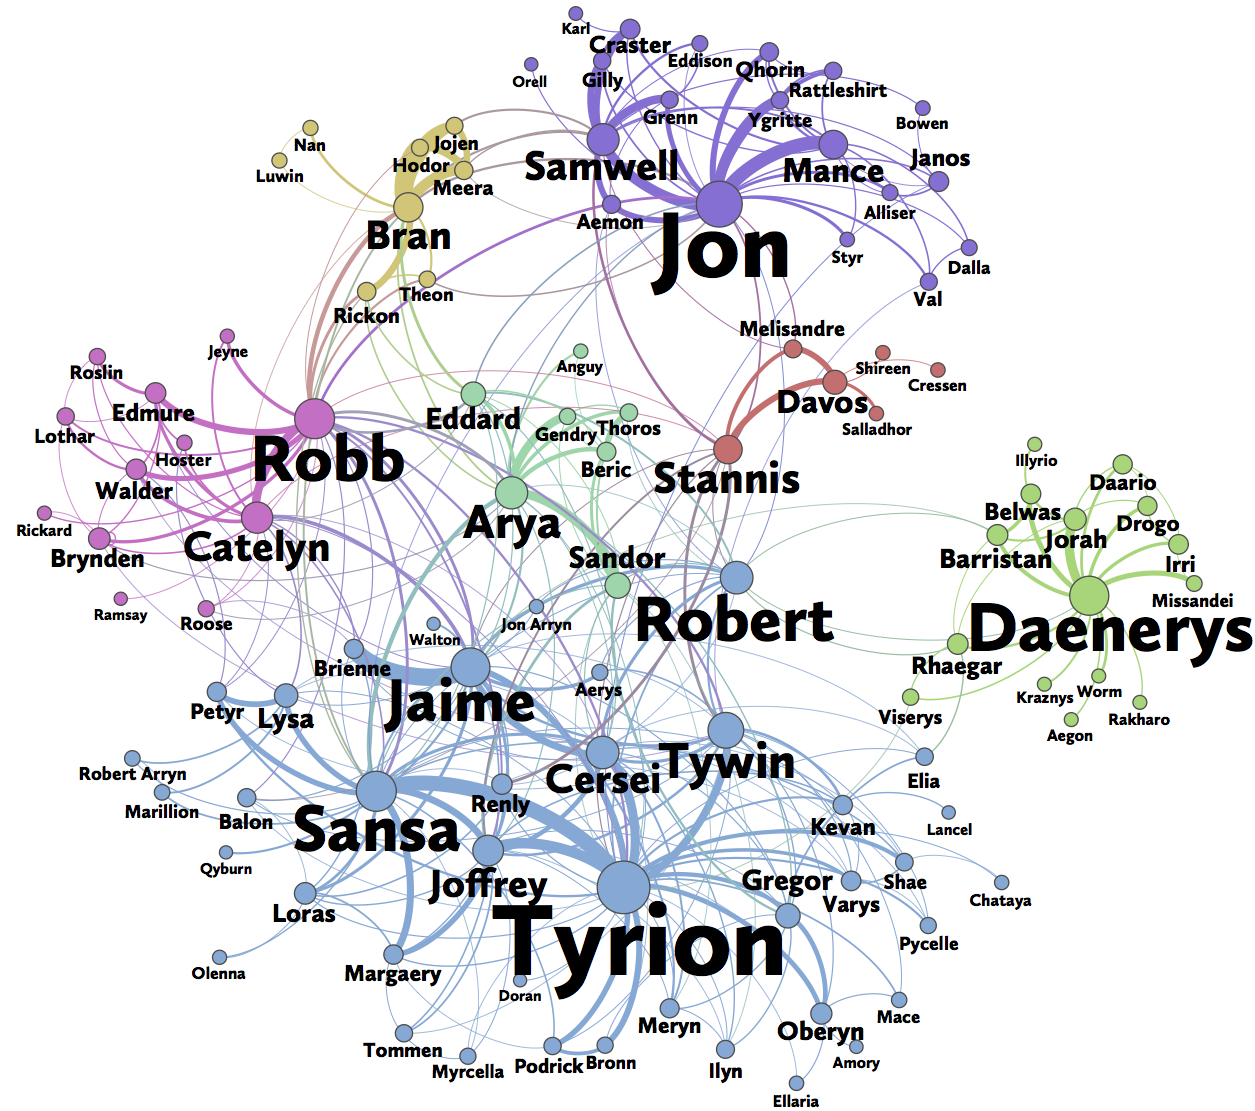
\includegraphics[width=0.75\textwidth]{Graphics/got-network.png}
    \caption{Game of Thrones social Network,\\
    Quelle: https://predictivehacks.com/social-network-analysis-of-game-of-thrones/,\\ Stand: 28.03.2022}
    \label{fig:GameOfThrones}
\end{figure}

Das Netzwerk besteht aus $796$ Knoten und $2823$ Kanten. Insgesamt daher aus $796$ Charakteren aus \textit{Game of Thrones (GOT)}.
In dieser \textit{sozialen Netzwerk Analyse} tauchen auch bisher unbekannte Messungen auf, die aber im Interpretations-Teil dieser Arbeit ebenfalls aufgegriffen werden. Beispielsweise beträgt der \textit{Durchmesser} des GOT Graphen $9$. Das heißt, wenn die kürzeste Pfadlänge von jedem Knoten zu allen anderen Knoten berechnet ist, ist der Durchmesser die längste aller berechneten Pfadlängen. Die durchschnittlich kürzeste Pfadlänge beträgt $3.41$. Diese wird aber zu einem späteren Zeitpunkt analysiert. In Abbildung \ref{fig:GameOfThrones} ist gut zu erkennen, welche Knoten eine zentrale Rolle in diesem spielen. Hierfür wird mit der Knoten-Größe in der Abbildung \ref{fig:GameOfThrones} variiert. Große Knoten implizieren, dass es sich um einen wichtigen Knoten in dem Teilgraphen handelt und kleine, dass es sich um weniger relevante Knoten handelt \cite{GOT}. 
\begin{table}[h!]
\footnotesize
\caption{Werte GOT Graph}
\label{TableGOT}
\begin{tabular}{lccccc}\toprule 
\textbf{Charakter} &\textbf{Grad-Zentr.} & \textbf{Charakter} &\textbf{Nähe-Zentr.}  & \textbf{Charakter} &\textbf{Betweeness-Zentr.} \\
 &\\\midrule
  Tyrion Lannister & 0.1535  & Tyrion Lannister & 0.4763 & Jon Snow& 0.1921   \\
  Jon Snow & 0.1434 & Robert Baratheon & 0.4593 & Tyrion Lannister & 0.1622   \\
  Jaime Lannister & 0.1270  & Eddard Stark& 0.4558& Daenerys Targaryen & 0.1184   \\
  Cersei Lannister & 0.1220 & Cersei Lannister & 0.4545 & Theon Greyjoy & 0.1113   \\
  Stannis Baratheon & 0.1119 & Jaime Lannister & 0.4520 & Stannis Baratheon & 0.1101   \\
       
  \\\bottomrule
 \end{tabular}
 \end{table}
Wenn diese Knoten in der Abbildung \ref{fig:GameOfThrones} gesucht werden, ist visuell direkt ersichtlich, dass es sich hierbei um die Knoten mit den meisten Verbindungen handelt. Oftmals ist leider bei den abgebildeten Graphen nicht eindeutig erkennbar, ob es sich hierbei um Kanten handelt, welche zwei Knoten direkt miteinander verbinden, oder die Kanten lediglich am Knoten vorbei verlaufen. Deshalb ist es wichtig, die Werte aus der Tabelle \ref{TableGOT} zu analysieren. Hier fällt bei den Spalten \textit{Charakter} auf, dass \textit{Tyrion -Lannister} in allen aufgeführt wird. Das heißt, dass dieser Knoten im Graphen (visuell betrachtet) sowohl zentral liegen, und zudem kurze Abstände zu den anderen Knoten nachweisen muss. Zudem müssen über diesen Knoten die häufigsten kürzesten Wege verlaufen. Bei der Abbildung \ref{fig:GameOfThrones} fällt ebenfalls auf, dass der Knoten, beziehungsweise Charakter, $Tyrion$  heraus sticht. Er ist von den meisten Knoten und Kanten umgeben. Da drei der fünf wichtigsten Knoten in der Spalte $Grad-Zentr.$ den gleichen zweiten Namen tragen, liegt die Vermutung nahe, dass es sich hier um Knoten handelt, die auch visuell betrachtet sehr nah beieinander liegen müssem. Beim Betrachten des Graphen bestätigt sich diese Vermutung direkt, denn alle drei Knoten befinden sich im blauen Teilgraphen. Zudem handelt es sich bei dem Namen $"Lannister"$ um ein Adelshaus in der US-amerikanischen Fantasy-Fernsehserie \textit{Game of Thrones} was die starke Verbindung und Nähe zueinander begründet. Außerdem fällt sofort auf, dass drei der fünf Charaktere in der Spalte \textit{Nähe-Zentr.} die selben sind, wie die wichtigsten Charaktere bezüglich der \textit{Grad-Zentr.} Wieder bedeutet das, dass diese Charaktere sowohl zentral im Graphen liegen müssen als auch die kürzesten Wege zu anderen Knoten besitzen. Die Betrachtung von Abbildung \ref{fig:GameOfThrones} bestätigt dies sofort. Zudem weist der Graph auch einige Cliquen auf. Die relevanteste und vor allem größte Clique befindet sich im blauen, grünen, ein Knoten im roten und zwei Knoten im pinken Teilgraphen. Aus dem Kapitel über Brücken und Cliquen \ref{ch:CliquenBrücken} ist bekannt, dass die Knoten mit den höchsten Zentralitäten höchstwahrscheinlich eine Clique darstellen und es sich vor allem bei den Knoten mit hohen \textit{Zwischen-Zentralität} um Brücken handelt. Jedoch wird die Analyse dieses sozialen Netzwerks nicht weitergeführt, sondern auf die Analyse des selbst generierten sozialen Netzwerks fokussiert. Auch auf die Frage, welcher mathematischen bzw. stochastischen Verteilung die Zentralitäten entsprechen und warum eine solche Untersuchung sinnvoll ist, wird zu einem späteren Zeitpunkt eine Antwort gegeben.

%*****************************************
%*****************************************
%*****************************************
%*****************************************
%*****************************************
